\chapter{Metodologia}

    % Como discutido anteriormente, as diferentes formas nas quais os dados censitários, bem como o de outras pesquisas como a Pesquisa Nacional por Amostra de Domicílios (PNAD), se diferem basicamente por seu formato, JSON para a API e 
    
    % Por conta das diferentes formas em que os dados se encontram disponibilizados pelo IBGE discutidas anteriormente, e também pelo caráter dos mesmos quanto à granularidade e quais dados são disponibilizados, foram tomadas duas diferentes abordagens: a de coletar os dados através da API de serviço de dados e a de baixar os arquivos de microdados dos Censos de 2000 e 2010 e transformá-los em dados 

    Como discutido anteriormente, as diferentes formas nas quais os dados censitários, bem como de outras pesquisas do IBGE, são disponibilizados, se diferem basicamente quanto ao seu grão e formato, sendo os agregados dis



    

\section{APIs do serviço de dados do IBGE}

    O IBGE disponibiliza em seu serviço de dados ao todo 17 APIs, incluindo a de Agregados, já discutida anteriormente, a de Localidades, que inclui os códigos dos vários níveis de localidade (p. ex. unidade federativa (UF), macrorregião, município), a de Metadados, incluindo informações como periodicidade e variáveis disponíveis em cada uma das pesquisas disponíveis na API, entre outras. Nestas APIs é possível, através de \textit{Uniform Resource Locators} (URLs) gerar requisições por meio de bibliotecas como a \textit{requests} do \textit{python} para obter os dados da API no formato \textit{Javascript Object Notation} (JSON). Por exemplo, se fizermos uma requisição a API de localidades utilizando a URL \url{https://servicodados.ibge.gov.br/api/v1/localidades/distritos} obteremos uma lista de valores no formato do exemplo \textit{Listing} \ref{lst:exemplo-api-localidades}:

    
    % EDITAR: uso de primeira pessoa!!!!!!!!!!!!!!!!!!


    \bigskip
    
\begin{lstlisting}[float = h, label={lst:exemplo-api-localidades},language=Python, caption=Exemplo de resultado de uma requisição da API de localidades.]
{"id":421400310, "nome":"Mirador",
  "municipio":{"id":4214003,"nome":"Presidente Getúlio",
    "microrregiao":{"id":42011,"nome":"Rio do Sul",
      "mesorregiao":{"id":4204,"nome":"Vale do Itajaí",
        "UF":{"id":42, "sigla":"SC","nome":"Santa Catarina",
          "regiao":{"id":4, "sigla":"S", "nome":"Sul"}}}},
    "regiao-imediata":{"id":420023, "nome":"Ibirama - Presidente Getúlio",
      "regiao-intermediaria":{"id":4207, "nome":"Blumenau",
          "regiao":{"id":4, "sigla":"S","nome":"Sul"}}}}
}
\end{lstlisting}


% {"id":420690010, "nome":"Dalbérgia",
%   "municipio":{"id":4206900, "nome":"Ibirama",
%     "microrregiao":{"id":42011, "nome":"Rio do Sul", "mesorregiao":{"id":4204, "nome":"Vale do Itajaí",
%         "UF":{"id":42, "sigla":"SC", "nome":"Santa Catarina",
%           "regiao":{"id":4, "sigla":"S", "nome":"Sul"}}}},
%     "regiao-imediata":{"id":420023, "nome":"Ibirama - Presidente Getúlio",
%       "regiao-intermediaria":{"id":4207, "nome":"Blumenau",
%         "UF":{"id":42, "sigla":"SC", "nome":"Santa Catarina",
%           "regiao":{"id":4, "sigla":"S", "nome":"Sul"}}}}}}

    Contudo a formatação JSON, por mais que seja mais eficiente de um ponto de vista transacional, não é ideal para o uso analítico por possuir como característica certa complexidade de navegação e maior custo computacional para criação de consultas, desta forma sendo melhor o armazenamento dos dados em formato tabular, já que persistência e normalização não são preocupações primárias quando refere-se a dados analíticos. Para tal, foi realizado o processo conhecido como \textit{unnesting} (desaninhamento em português), onde os dados de um certo nível de aninhamento são trazidos recursivamente para seu nível superior até que estejam todos em um único nível. O algoritmo em \textit{listing} \ref{lst:unnesting} demonstra como é realizado o processo de \textit{unnesting}:

\bigskip

\begin{lstlisting}[float = h, label={lst:unnesting},language=Python, caption=Algoritmo de \textit{unnesting} em \textit{python}.]
def unnest_json(json_dict: dict, col_name: str = '') -> dict:
    output = {}
    # Define uma função recursiva que "achata" (flatten) o JSON
    def flatten(column, col_name:str = ''):
        # Checa se a coluna é do tipo dict e continua a recursão se sim
        if type(column) == dict:
            # Itera sobre as chaves do dicionário
            for key in column:
                # Determina o nome da coluna para a chave (key) atual
                if col_name == '':
                    new_col_name = str(key)
                else:
                    # adiciona o nome do pai da coluna ao nome da coluna
                    parent_col = col_name.split('_')[-1]
                    new_col_name = parent_col + '_' + str(key)
                # Chama recursivamente a função flatten para a chave (key) atual
                flatten(column[key], new_col_name)
        else:
            # Se a coluna não é do tipo dict, salva o valor dela no output
            output[col_name] = column
    # Chama a função de flatten usando o JSON como parâmetro
    flatten(json_dict, col_name)
    return output
\end{lstlisting}

    Após o \textit{unnesting} feito, obtemos os dados todos em um mesmo nível, sendo assim capazes facilmente de transformá-los em uma tabela como a exemplificada pela tabela \ref{tab:exemplo-api-localidades}:

\begin{center}
    \begin{table}[h]
        \begin{tabular}{c l c l c l}
            \hline
                id-distrito & nome-distrito & id-municipio & nome-municipio & $\dotsi$ & nome-regiao\\
            \hline
                421400310 & Mirador & 4214003 & Presidente Getúlio & $\dotsi$ & Sul\\
                420690010 & Dalbérgia & 4206900 & Ibirama & $\dotsi$ & Sul\\     
            \hline
        \end{tabular}
        \caption{Exemplo dos dados de localidade em formato tabular. Fonte: Dados do autor (2023).}
        \label{tab:exemplo-api-localidades}
    \end{table}
\end{center}

    Um certo problema que pode ainda ocorrer é que, mesmo após o \textit{unnesting}, que os dados em JSON podem conter também elementos em formato de lista, gerando assim uma coluna na tabela de resultado que possui em si uma lista de valores. Portanto se faz necessário um segundo tratamento para estes casos, que é facilmente resolvido armazenando o conjunto de dados dentro de um objeto do tipo \textit{DataFrame} da biblioteca \textit{pandas} da linguagem \textit{python} e utilizar o método \lstinline{pandas.DataFrame().explode()}\footnote{Documentação disponível em <\url{https://pandas.pydata.org/docs/reference/api/pandas.DataFrame.explode.html}>, código fonte disponível em <\url{https://github.com/pandas-dev/pandas/blob/v2.1.1/pandas/core/frame.py\#L9432-L9558}>. Acessado em 30 de set. 2023.}     de modo a converter elementos \textit{list-like} que possam existir dentro das colunas em linhas, copiando os demais valores, como é exemplificado pela figura \ref{fig:exploding-df}.

\begin{figure}[h]
    \centering
    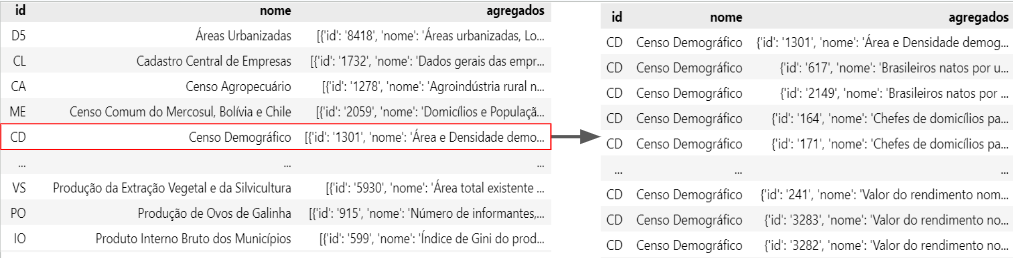
\includegraphics[width=\textwidth]{files/img/exploding_table.png}    \caption{Exemplo do uso do método \lstinline{pandas.DataFrame().explode()}. Fonte: Dados do autor (2023).}
    \label{fig:exploding-df}
\end{figure}

    Nota-se que os valores ``explodido'' continuam aninhados, portanto nesse caso foi necessário reaplicar a função \lstinline{unnest_json()} de modo a separar adequadamente os dados.

    [Adicionar: como fiz a carga de localidades, como fiz a carga dos países, procedimento para criar a URL adequada para a carga dos agregados]



\section{Microdados do Censo Demográfico}

    Os dados fornecidos pela API de agregados consistem essencialmente na consolidação das respostas individuais de cada um dos entrevistados durante o processo de recenseamento de acordo com critérios locacionais, com seu menor grau de agregação sedo município. Tais informações são organizadas em um formato denominado pelo IBGE como microdados e são disponibilizados através do portal de produtos estatísticos da instituição\footnote{Para mais detalhes, consulte <\url{https://www.ibge.gov.br/estatisticas/todos-os-produtos-estatisticas.html}>. Acesso em 03 out. 2023}, estando disponibilizados em diversas pastas compactadas em formato \textit{.zip} que contém os arquivos de texto nos quais se encontram os dados. No entanto, os dados daqueles arquivos não estão imediatamente prontos para a utilização tal qual uma planilha ou um arquivo CSV, mas sim em um formato comprimido, onde os valores categóricos são codificados através de identificadores (IDs) numéricos, enquanto valores que originalmente possuíam casas decimais tem seus pontos flutuantes removidos. Dessa forma, os dados se apresentam conforme ilustrado pela figura \ref{fig:exemplo-microdado}:

\begin{figure}[h]
    \centering
    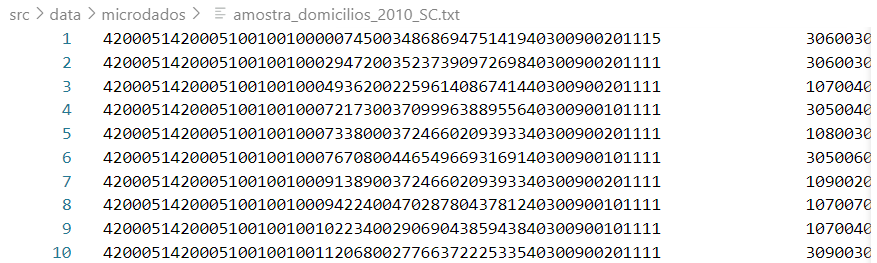
\includegraphics[width=\textwidth]{files/img/exemplo_microdado.png}
    \caption{Exemplo de microdados: primeiras 10 linhas da pesquisa de Domicílios do Censo de 2010 no estado de Santa Catarina. Fonte: Dados do Autor (2023).}
    \label{fig:exemplo-microdado}
\end{figure}

    Juntamente com os microdados, é fornecido uma planilha no formato \textit{Open Document Spreadsheet} (ODS) ou Excel que descreve o que cada caractere do arquivo significa, relacionando as categorias e identificadores e a formatação referente às casas decimais das variáveis numéricas. 
    
    Tomando como exemplo a amostra da pesquisa de domicílios do Censo Demográfico de 2010, o arquivo de \textit{layout}\footnote{\label{fn-layout-domi}Arquivo /Documentação/Layout/Layout\_microdados\_amostra.xls. Download em: <\url{https://ftp.ibge.gov.br/Censos/Censo_Demografico_2010/Resultados_Gerais_da_Amostra/Microdados/Documentacao.zip}>. Acesso em 03 out. 2023.} (exemplificado na figura \ref{fig:layout-domi}), temos que as duas primeiras posições do arquivo referem-se variável V0001 à UF, cujo valor 42 corresponde ao Estado de Santa Catarina. Outro exemplo significativo é a variável numérica V0010, Peso Amostral, engloba os dígitos da posição 29 até 44, sendo os 3 primeiros (coluna INT) os dígitos anteriores ao ponto decimal, e as 13 subsequentes sendo as casas de precisão após a vírgula (coluna DEC).

\begin{figure}[h]
    \centering
    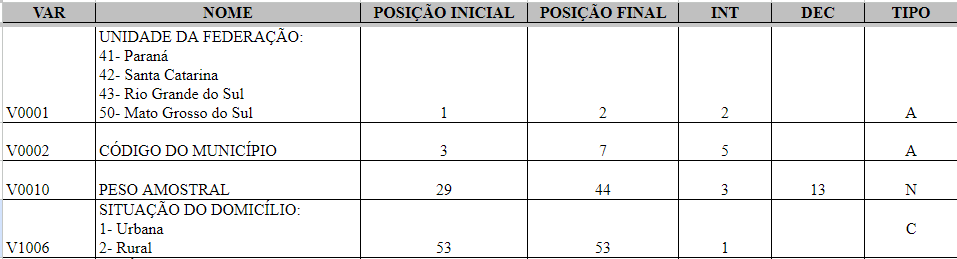
\includegraphics[width=\textwidth]{files/img/layout amostra domicilios 2010.png}
    \caption{Recorte da planilha de \textit{layout} da pesquisa de domicílios do Censo Demográfico de 2010. Fonte: Dados do Autor (2023).}
    \label{fig:layout-domi}
\end{figure}

    Variáveis padrões contidas nas pesquisas são as referentes à localização geográfica como município, UF e área de ponderação, assim como o peso amostral, que por sua vez é uma medida de representatividade daquela resposta dentro do escopo da pesquisa.

    De modo a preparar os microdados para que estes possam ser utilizados, foi utilizado o \textit{software} Stata (em sua versão 18.0) para associar os IDs e respectivos valores descritos no arquivo de \textit{layout} e então gerar um arquivo de dados que posteriormente poderá ser utilizado como \textit{dataset}. 
    Com comandos do Stata é possível definir a posição em que se encontram as informações de cada variável, sua tipagem, suas \textit{labels} e respectivos pares chave e valor, para então o arquivo de dados ser processado, que é exemplificado pelo \textit{Listing} \ref{lst:do-file-sample} a seguir:

\bigskip
\begin{lstlisting}[float = h, label={lst:do-file-sample},language=Stata, caption=Exemplo de comandos Stata utilizados para``traduzir'' os microdados.]
* Define as posições onde se encontram cada dado
quietly infix                         ///
  byte		V1006		53-53		///
  double		V6204		82-84		///
using `"amostra_domicilios_2010_RJ.txt"', clear
* Define a formatação dos dados numéricos
* Neste caso,  o dado deve assumir a formatação 0000.0
format V6204 %04.1f
* Define as labels para os dados
label var V1006		`"SITUAÇÃO DO DOMICÍLIO"'
label var V6204		`"DENSIDADE DE MORADOR / DORMITÓRIO  "'
* Define os pares chave-valor para cada variável
label define V1006_lbl 1 `" Urbana"', add
label define V1006_lbl 2 `" Rural"', add
* Associa os valores da variável V1006 com os pares chave-valor armazenados em V1006_lbl
label values V1006 V1006_lbl
\end{lstlisting}

    O exemplo acima nada mais é que um pequeno recorte do arquivo completo da pesquisa de domicílios, que conta com 76 variáveis e mais de 6 mil \textit{labels}, já que as variáveis de caráter locacional pode se referir a qualquer um dos mais de 5 mil municípios do país e suas respectivas regiões. 
    
    Como facilitador para tal associação de pares chave-valor, foi desenvolvido um código \textit{python}\footnote{Código disponível em <\url{https://github.com/GDevigili/DW-IBGE/blob/main/src/notebooks/gera-script-stata.ipynb}>.} que gera um \textit{script} para ser utilizado pelo Stata para o processamento  ``tradução'' dos microdados. 
    Primeiramente, através das colunas de posição inicial e final, mapeamos os caracteres que representam cada uma das colunas do conjunto de dados, então foi adicionada a formatação adequada para os dados numéricos com o comando \verb|format|. Posteriormente são definidos os nomes das colunas com o comando \verb|label define| e então associados os pares chave-valor, extraídos de um \verb|DataFrame| pré processado com os dados presentes no arquivo de \textit{layout}. Os valores correspondentes aos municípios, microrregiões, mesorregiões e regiões metropolitanas se encontram em arquivos auxiliares, porém foi optado por utilizar a própria API de localidades para obter os respectivos valores já que o trabalho para a extração de dados já havia sido realizado anteriormente.


\chapter{Estudo de Caso}